%%%%%%%%%%%%%%%%%%%%%%%%%%%%%%%%%%%%%%%%%
% Structured General Purpose Assignment
% LaTeX Template
%
% This template has been downloaded from:
% http://www.latextemplates.com
%
% Original author:
% Ted Pavlic (http://www.tedpavlic.com)
%
% Note:
% The \lipsum[#] commands throughout this template generate dummy text
% to fill the template out. These commands should all be removed when 
% writing assignment content.
%
%%%%%%%%%%%%%%%%%%%%%%%%%%%%%%%%%%%%%%%%%

%----------------------------------------------------------------------------------------
% PACKAGES AND OTHER DOCUMENT CONFIGURATIONS
%----------------------------------------------------------------------------------------

\documentclass[12pt]{article}

\usepackage{fancyhdr} % Required for custom headers
\usepackage{lastpage} % Required to determine the last page for the footer
\usepackage{extramarks} % Required for headers and footers
\usepackage{graphicx} % Required to insert images
\usepackage{lipsum} % Used for inserting dummy 'Lorem ipsum' text into the template
\usepackage{wrapfig}
\usepackage{enumitem}
\usepackage{subcaption}

\usepackage[explicit]{titlesec}

\usepackage[export]{adjustbox}

% Margins
\topmargin=0in
\evensidemargin=0in
\oddsidemargin=0in
\textwidth=6.5in
\textheight=9in
\headsep=0.5em 

\linespread{1} % Line spacing

% list spacing
\setlist{nosep}

% caption spacing
% \setlength\belowcaptionskip{-3pt}

% \bibliographystyle{plain}

\titleformat{\section}
  {\bfseries}{\thesection}{0em}{#1}
\titlespacing*{\section}{0em}{0em}{0em}[0em]

% Set up the header and footer
\pagestyle{fancy}
\lhead{\AuthorName} % Top left header
\chead{\Title} % Top center header
\rhead{\Subject} % Top right header
\fancyfoot{}
% \lfoot{\lastxmark} % Bottom left footer
% \cfoot{} % Bottom center footer
% \rfoot{Page\ \thepage\ of\ \pageref{LastPage}} % Bottom right footer
\renewcommand\headrulewidth{0.4pt} % Size of the header rule
% \renewcommand\footrulewidth{0.4pt} % Size of the footer rule

\setlength{\parskip}{0.3em}
\setlength\parindent{10pt} % Removes all indentation from paragraphs


\newcommand{\Title}{Project Narrative} % Assignment title
\newcommand{\Subject}{NSTRF 2016}
\newcommand{\AuthorName}{Colin Rennie} % Your name

\begin{document}
\newpage

\begin{center}
{\bf Coordinated Planning and Control for Tethered Robot Pairs }

\end{center}

%---------------- Introduction ------------------
%Tethered Robot Importance 
%Planetary exploration
%Situations needing tethers for science targets
%Communications
Many important and rewarding science target locations on extra-planetary bodies lie in terrain that is 
rocky, uneven, or involves traversing steep inclines in order to access. Consider the search for ice in 
underground caves on Mars, or collecting soil samples and images from the bottom of a crater or ravine. 
These tasks, while very rewarding in terms of scientific value, are not easily achieved by humans nor 
the current generation of planetary rovers. This shortcoming of current exploratory technology has spurred 
considerable interest in the development of next generation rover designs featuring a tether that either 
connects the rover to a static point in the environment or, even more desirably, connects to another rover 
vehicle of equal capabilities. A tethered pair of robots not only benefits from the stability that a tether 
provides while rappelling down difficult terrains, but has added robustness benefits from having an additional robot 
at its disposal. For example, the base robot can reconfigure to provide maximal stability, it can descend down in order to help 
in case of immobility, and the pair can swap roles between (1) providing stability to the other and (2) traversing the 
terrain, allowing the tethered pair to safely traverse difficult terrain well beyond what a single anchored robot 
could achieve. 

\begin{wrapfigure}{r}{0.5\textwidth}
  % \begin{center}
  \vspace{-0.2in}
  \begin{subfigure}{.245\textwidth}
    \centering
    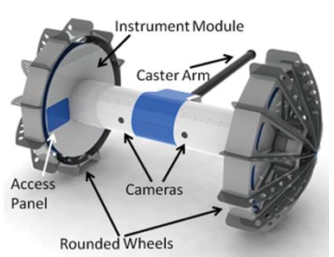
\includegraphics[width=.75\linewidth]{axel_prototype}
    \caption{}
    \label{fig:axel}
  \end{subfigure}%
  \begin{subfigure}{.245\textwidth}
    \centering
    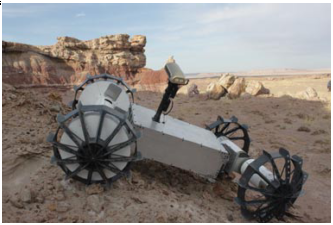
\includegraphics[width=.95\linewidth]{duaxel_prototype}
    \caption{}
    \label{fig:duaxel}
  \end{subfigure}
  \begin{subfigure}{.245\textwidth}
    \centering
    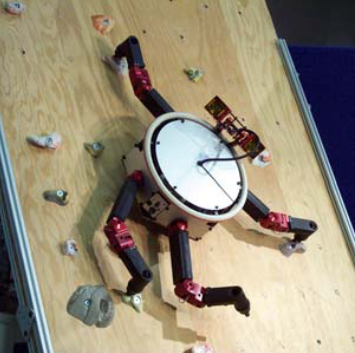
\includegraphics[width=.88\linewidth]{lemur_prototype}
    \caption{}
    \label{fig:lemur}
  \end{subfigure}%
  \begin{subfigure}{.245\textwidth}
    \centering
    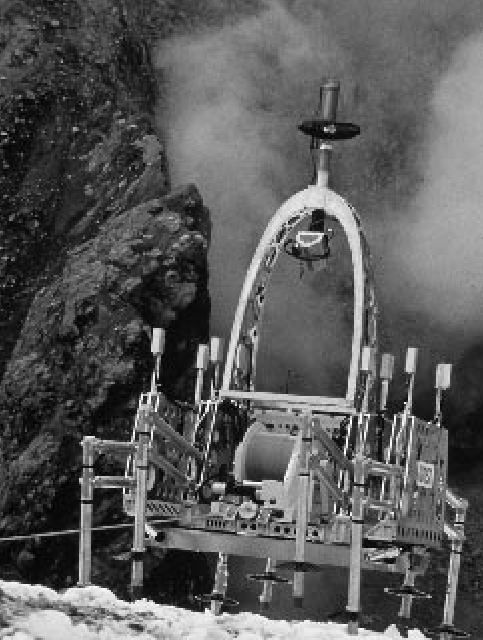
\includegraphics[width=.65\linewidth]{dante_prototype}
    \caption{}
    \label{fig:dante}
  \end{subfigure}  % \end{center}
  \label{fig:prototypes}
  \vspace{-0.1in}
  \caption{(a) The Axel II rover prototype (b) Two Axel II rovers in DuAxel configuration 
  with support structure (c) Lemur IIb autonomous climbing robot (d) Dante II robot exploring a 
  volcanic crater. }
\end{wrapfigure}

In this proposal we present an overview of the state-of-the-art in tethered robots designed with the goals 
mentioned above in mind and cover recent developments in motion planning for this difficult problem. 
We then propose two related research problems, viable solutions to which we believe would tremendously aid 
in the utility of tethered robot technology: a control strategy for re-configuring the tether between two 
rovers in order to deal with unforeseen challenges in the terrain, and a planning problem which uses this 
control strategy as a ``submodule'' while planning for coordinated descent/ascent of difficult terrain with 
a tether constraint. Solutions to these problems as we present them would be platform-independent, but could 
apply well beyond the scope of extra-planetary exploration. For example, it could be beneficial to attach a 
tether to Robonaut in case an emergency retraction is needed as it navigates the International Space Station. 
With the help and support of NASA's STRF program, we propose to work on these problems for the duration of our 
studies. 


%----------------------------------------------
%---------------- Background ------------------
%----------------------------------------------

{\bf\noindent Tethered Rover Systems Background}

Recent research into robot designs for the traversal of harsh and difficult terrains 
has featured several very different designs with different means of locomotion. Several of these systems 
include an actuated winch or spooled tether used for communication and/or stability while locomoting. 
Notable examples include an eight-legged walking robot attached to a stationary base [Fig. \ref{fig:dante}] and a pair of 
two-wheeled differential drive robots connected with a soft tether [Fig. \ref{fig:duaxel}]. Even more novel recent 
robot designs could benefit from the presence of a tether attachment to an exploratory counterpart. We believe 
this list to include Lemur IIb, a four-legged climbing robot [Fig. \ref{fig:lemur}], which could potentially use an actuated 
tether to swing its counterpart onto protruding overhangs and then, in turn, rappel from the stabilized counterpart robot 
in order to reach the overhang safely.

%Dante II (& lemur II?)
The Dante II robot design consisted of eight legs for locomotion and an 
actuated winch used for rappelling down steep and difficult terrain from a static anchor point. 
Both actuation mechanisms were attached to 
a base frame with a sensor arch protruding from the top of the structure \cite{dante_design}. A variety of
sensing equipment, including a pan/tilt camera and a laser range finder,
 were attached to the arch in order to retrieve and transmit data from remote
 locations. In 1994 the system was deployed into Mount Spurr, an active volcanic site, 
 in order to record data for further scientific analysis. The robot's control 
 during this time was a combination of supervised autonomous motions and remote
 teleoperation \cite{dante_results}. During the mission the robot suffered from a failure 
 where the robot incurred a lateral force at its contact
point with the tether, fell over, and was not able to correct itself. Apart from this occurrence, however, 
the 5-day mission was regarded as a success in showing the capabilities of robotic systems to act as ``surrogate scientists''; exploring where humans would not otherwise be able. 

\begin{wrapfigure}{r}{0.5\textwidth}
  \vspace{-0.4in}
  \begin{subfigure}{.45\textwidth}
    \centering
    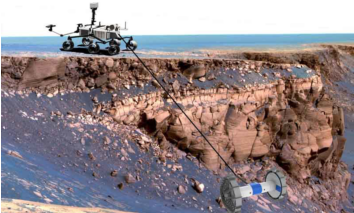
\includegraphics[width=.95\linewidth]{axel_deploy}
    \caption{}
    \label{fig:axeldeploy}
  \end{subfigure}\\
  \begin{subfigure}{.25\textwidth}
    \centering
    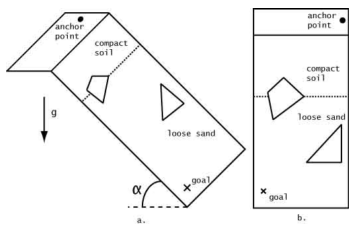
\includegraphics[width=.99\linewidth]{planar_terrain}
    \caption{}
    \label{fig:planarterrain}
  \end{subfigure}%
  \begin{subfigure}{.2\textwidth}
    \centering
    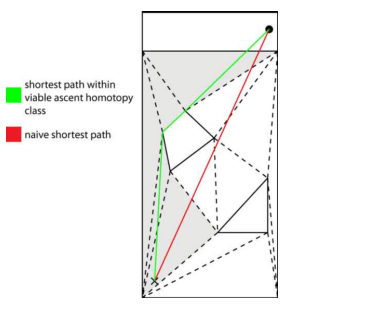
\includegraphics[width=.95\linewidth]{planar_path}
    \caption{}
    \label{fig:planarpath}
  \end{subfigure}  % \end{center}
  \label{fig:dsolution}
  \vspace{-0.1in}
  \caption{(a) Conceptualized descent terrain for Axel II mission (b) example projection of terrain to 2D plane
  (c) example solution: viable controllable regions for ascent (shaded), naive shortest path (red), shortest path within 
  viable homotopy class (green). }
\end{wrapfigure}

%Axel platform (+picture)
More recently, NASA's Jet Propulsion Laboratory has been working on a two-wheeled
differential drive tethered robot, appropriately named ``Axel''. The Axel II robot 
design features collapsible, paddled wheels, making the system more appropriate for longer 
and more remote missions as this design is more robust to issues such as high-centering and 
failures such as that encountered by Dante II \cite{axel_design}. The tether mechanism is connected to the axle 
between the two wheels and is actively spooled as the wheels move relative to the body of the robot. 
Two variants of the system are presented: one in which Axel is attached to a stationary anchor point, 
and a second where two Axel robots are tethered together and deployed via a central support beam (``DuAxel'') \cite{duaxel}. 

%Motion planning solution
The open question in either design variation is how to plan autonomous descent and corresponding 
ascent paths for the deploying tethered Axel robot in uneven, rocky, extra-planetary terrains. 
A solution framework is presented which projects this complex problem to a two-dimensional plane and, 
building on foundational work addressing the tether constraint problem from a computational geometry 
perspective \cite{ties_that_bind, min_homotopies}, extends this approach to produce ``controllable'' 
paths by deriving equations of 
motion arising from the constraints of the Axel robot \cite{axel_planning}. 
The planning problem the authors address in this work is of planning a single mission, consisting of 
a descent and corresponding ascent, while being stabilized by tether attachment to a static anchor point. 
The resulting algorithm first plans the more difficult ascent path and then 
uses the solution to limit its search for viable descent paths lying in the same homotopy class. 

%Problems
%   Quasi-static, no cable friction with ground assumed
%   solution is planar, over-simplifying the environment
%   assumes static anchor point (base unit)
While this solution represents substantial progress well-grounded in foundational work, the 
assumptions and simplifications made leave much to be desired in terms of robust autonomous
exploration. Projecting these types of difficult three-dimensional terrain environments in two-dimensions and representing obstacles as simple polygons [Fig. \ref{fig:planarterrain}] is not a realistic strategy for complex extra-planetary terrains. 
This strategy makes the additional assumptions of prior perfect knowledge of the environment, frictionless 
interaction of the tether with the ground plane, and quasi-static motion of the robot. 
Most relevant to the work proposed in the next section is that is remains an open question as to how 
best to plan autonomous motions for the DuAxel configuration where two 
dynamic robots take turns belaying each other.

%-----------------------------------------------------
%---------------- Proposed Research ------------------
%-----------------------------------------------------

% Doing so allows us to plan in a 
% kinodynamic way (taking into account constraints on velocity and acceleration of the robot) and generate solutions which 
% account for the robot's dynamics (as opposed to quasi-static solutions)
{\bf\noindent Proposed Research}

{\sl The main goal of this research is to address the problem of planning for tethered pairs of exploratory 
robots in their full three-dimensional workspace, i.e., without projecting the problem to a lower dimension. 
Our solution provides a control strategy for addressing unforeseen obstacles and failures, and uses this strategy 
as a submodule in planning paths for tethered pairs of robots in which the robots alternate exploring and providing 
support to their counterpart.}

In this proposal, we consider a tethered pair of robots of arbitrary design. As such, our approach is applicable 
to any tethered pair of rovers provided that they have a means of: (1) actuating the tether at its contact points with 
each rover and (2) measuring the forces exerted on each rover at the tether's contact points. Likely the most similar system 
that we've presented so far in this proposal is the DuAxel design, which fits these specifications already. However, one can 
also apply this approach to a pair of Lemur IIb robots free-climbing a vertical and jagged cliff face or even a pair of traditional 
wheeled rovers descending a steep and rocky mountainside. 

%---------------- Research Problem 1 ------------------

\noindent\underline{Research Problem 1: Coordinated control of a soft tether}

{\sl Goal: In presence of imperfect terrain information, we require a strategy for dealing with both 
unforeseen obstacles and unplanned tether snags on rocky elements of the terrain. }

% Outline the problems
In the following, we consider several potentially difficult situations that are likely 
to arise when planning for a tethered pair under imperfect information about the terrain. In 
addressing this problem in the full 3D workspace, we 
require a strategy which can deal with two important potential failure cases. First, while performing the exploratory role, a rover 
encounters an unknown obstacle obstructing its planned path, which we'll call the 
``reevaluation'' case (addressed in the planar case in \cite{axel_online}).
Second, while the exploratory rover is moving along its planned obstacle-free path, the tether comes in contact with and 
becomes entangled on uneven terrain (the ``snagging'' case).

\begin{wrapfigure}{r}{0.5\textwidth}
  \begin{center}
    \vspace{-0.4in}
    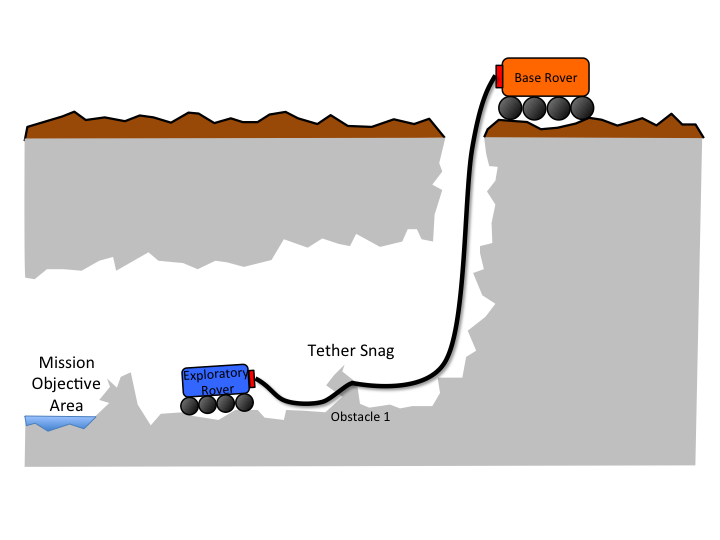
\includegraphics[width=0.48\textwidth, right]{cave_exploration}
  \end{center}
  \vspace{-0.4in}
  \caption{During a coordinated descent down a rocky extra-planetary surface, the tethered rover pair encounters an unplanned 
  snag of the tether with a rock in the terrain. The situation is resolved by using the coordinated wave-inducing control strategy to free 
  the tether.}
  \label{fig:tethersnag}
\end{wrapfigure}
% reevaluation case
In the snagging case [Fig. \ref{fig:tethersnag}], we propose to develop a low-level control law capable of inducing a 
traveling wave in the tether by employing 
an oscillatory control policy at the actuated tether contact of the rover closest to the tether snag's location. This approach is then 
similar to the strategy used by humans when they encounter the same situation while mountain climbing. 
The challenge in this strategy however, is that once the tether is free it's likely to impart a substantial 
force on the robot's stabilizing counterpart, potentially resulting in dangerous jerking in a partially known environment. 
A promising solution to this problem would be to induce in response a counteracting wave from the stabilizing rover's actuated tether 
contact. To this end, we would propose to explore first building a model (potentially analytically)
of the expected forces on the counterpart robot. We would then use this model in, e.g., a model predictive control-based solution where 
the low-level control policy optimizes its current control with respect to counteracting the incurred force over 
a finite time horizon of future predictions. It could also be advantageous to explore model-free approaches 
(e.g., designing an admittance controller), as it's possible that reacting to forces incurred is a more feasible 
solution than accurately predicting them ahead of time. 

% integration case: online re-planning wrt coordination between avoidance control and motion planning algo
In the reevaluation case of encountering an unmodeled obstacle in our path, what we must first decide is whether 
or not we can configure our tether such that we are able to place the tether in an arbitrary configuration on either side of the obstacle 
once we have moved past it. The reason we need to know this before moving forward is that while the unmodeled obstacle may not cause 
significant problems for our current rover's descent, planning the current stabilizing rover's traversal of the same slope is much more 
constrained as it does not have a stabilizing tether. Being able to place the tether on either side of the obstacle would then 
allow us to first plan the descent of the current stabilizing rover (incorporating this new obstacle), 
and then use the traversing rover to place the tether on the side of the obstacle that is easiest for the stabilizing rover to traverse. 

There are two tools at our disposal to determine whether this new obstacle is surmountable. By considering the height of the obstacle, 
we can search for configurations of the tethered pair which raise the tether above the obstacle, treating this as a planning subproblem. 
Alternatively, we can extend our snagging strategy outlined above -- simulating the effects of various parameterization of our 
wave-inducing control policies to find one that would be able to surmount the obstacle. If we successfully find such a policy, we can then 
combine this policy with a motion plan to move the exploratory rover to the desired side of the new obstacle, terminating the control policy 
once we've successfully reached the target state.

%---------------- Research Problem 2 ------------------

\noindent\underline{Research Problem 2: Motion planning for dynamic tethered rover pairs }

{\sl Goal: Integrating the control strategy outlined above as a subroutine in cases of environmental obstacles and tether 
entanglements, we aim to develop a robust motion planning framework for a tethered pair of rovers. This framework will be capable 
of planning the coordinated traversal of difficult terrain while the rovers alternate exploratory and stabilizing roles. }

\begin{wrapfigure}{r}{0.5\textwidth}
  \begin{center}
	\vspace{-0.4in}	
	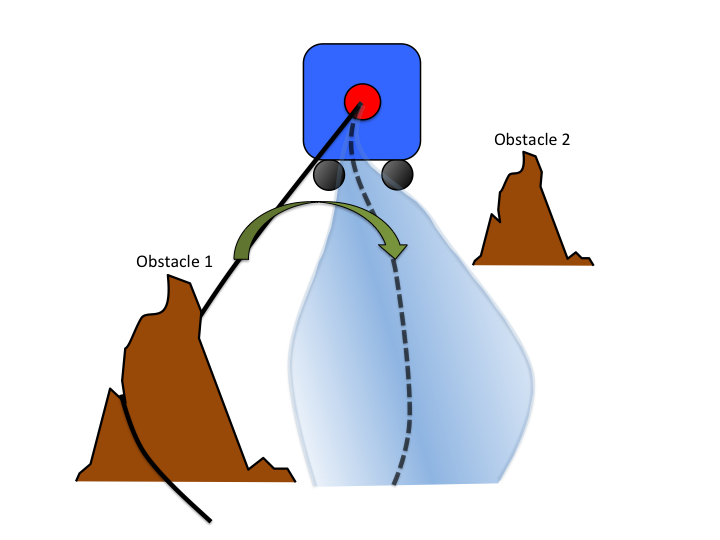
\includegraphics[width=0.48\textwidth, left]{cable_uncertainty}
  \end{center}
  \vspace{-0.2in}
  \label{fig:cable}
  \caption{Employing coordinated control between base and exploratory rovers, we are able to relieve the snagged cable 
  (green arrow) but in doing so are left with uncertainty about where the cable now lies (blue region).}
\end{wrapfigure}
Making use of the control strategy presented above when faced with unforeseen obstacles and situations, 
we can now outline our strategy for robustly
solving the motion planning problem of the coordinated traversal (ascent or descent) of difficult and partially known 
extra-planetary terrain. Beginning with our (incomplete) knowledge of the environment, we first select a set of maximally stable waypoints 
throughout the terrain. We then proceed iteratively and in an alternating fashion, first planning the descent of one of the rover
pair to the first stable waypoint, 
then the other to some next stable waypoint closer to the goal. The waypoints can then be thought of as ``role reversal''
locations. In this context, we call upon our control strategy as a submodule for dealing with unforeseen obstacles when 
they arise between a set of waypoints and then we re-plan. Importantly, re-planning under this strategy only requires re-computing 
the path between the current set of waypoints, as opposed to the trajectory of the entire traversal. 

%Solution Sampling-based
Planning between two waypoints in the full 3D workspace and taking into account the dynamics of the tethered system can be 
addressed using traditional sampling-based motion planning methods, which have been successfully applied to solve similarly 
high dimensional problems \cite{zak_kino}. The typical complaint with these methods, however, is the required time and 
computation required to randomly sample enough points to converge to a solution. Considering that we require our 
methods to be able to re-plan in a variety of situations, our desire is to substantially decrease the amount of time 
required to find solutions while still addressing this problem in its full state space. 

%Solution 
Several techniques can be drawn upon in such a scenario. The first set of approaches involve biasing the sampling of states 
in ways that utilize our in-depth knowledge of the problem we desire to solve. For example, by computing the ``most stable'' support 
position of the stabilizing rover (i.e., perpendicular to the current position of the exploratory rover or first encountered wrapped obstacle) 
and biasing our sampling toward samples that lie in this space. We would propose to additionally explore whether or not 
it is effective to solve this problem in a 2D projection first, then define a mapping from 2D space back to the full state space, 
and use this solution to bias samples in the full space. 

Additionally, we would explore the possibility that by dissecting the problem into multiple subproblem manifolds we can achieve reliable 
solutions much faster than in the full space. This has been achieved through use of machine learning techniques, where the authors 
train a model to learn the important sub-manifolds of a particular system's state space while also learning to predict which static 
configurations for other state dimensions would be most effective for solving the current problem \cite{learning_biases}. 








% ----------------end of document body---------------------

%---------------- start of references------------------
\newpage
\bibliographystyle{ieeetr}
\small{\bibliography{bibl.bib}}

%---------------- end of references------------------


\end{document}
